% !TeX spellcheck = it_IT
Questo capitolo tratta il passo successivo, ovvero la progettazione e lo sviluppo dell'applicativo facendo riferimento al caso d'uso descritto. Per motivi di tempo legati alle richieste del cliente, nell'applicazione dimostrativa  vengono tralasciate le questioni che concernono la sicurezza dei dati.

\section{Ambientazione Grafica}
Particolare attenzione è stata riposta nella progettazione dell'ambientazione 3D e nella scelta dei modelli. Questa parte infatti non solo è ciò che l'utente vede, come può essere la grafica di un'applicazione 2D, ma venendo immerso in questo ambiente, ne aumenta l'importanza e amplificando i feedback dell'utente. Ho infatti progettato insieme al collega addetto alla modellazione 3D l'ambiente utilizzando un approccio molto simile a quello impiegato nello studio di design d'interni.\\
Siamo partiti da delle immagini di riferimento rappresentanti sale riunioni moderne, senza particolari troppo caratteristici, mantenendo uno stile neutro e impersonale, soprattutto nella scelta dei colori e della mobilia virtuale.\\
Durante lo sviluppo di applicazioni per il Gear VR è fondamentale tenere in considerazione che il prodotto la limitata potenza di calcolo dei cellulari compatibili, in buona parte già impegnata nel gestire la simulazione virtuale. Come dispositivo per i test infatti è stato utilizzato il cellulare meno potente in termini di processore, ovvero il Samsung S6. Per evitare effetti sgradevoli su questi dispositivi è necessario ottimizzare al meglio l'applicazione e soprattutto i modelli 3D.\\
Per prima cosa bisogna eliminare ogni faccia geometrica dai modelli che non verrà mai visualizzata, poiché non vogliamo sprecare risorse renderizzando qualcosa che non verrà mai visto. Anche i modelli devo contenere il numero minimo di poligoni (\textit{low poly}) e di dettagli semplificando al massimo le mesh. Nel caso del nostro progetto la sfida risiedeva nell'ottenere un'ambientazione che nonostante fosse low poly, avesse uno stile realistico e formale, in contrasto con lo stile "cartoonesco" dei modelli 3D con pochi poligoni. Questo è stato possibile attraverso l'aggiunta dei dettagli, anziché sui modelli, sulle texture, utilizzando \textit{normal} e \textit{bump} maps di alta qualità e tramite la creazione di \textit{atlas} che unificassero queste ultime riducendo i loro tempi di carico e scarico della sulla memoria. 
\begin{figure}[H]
	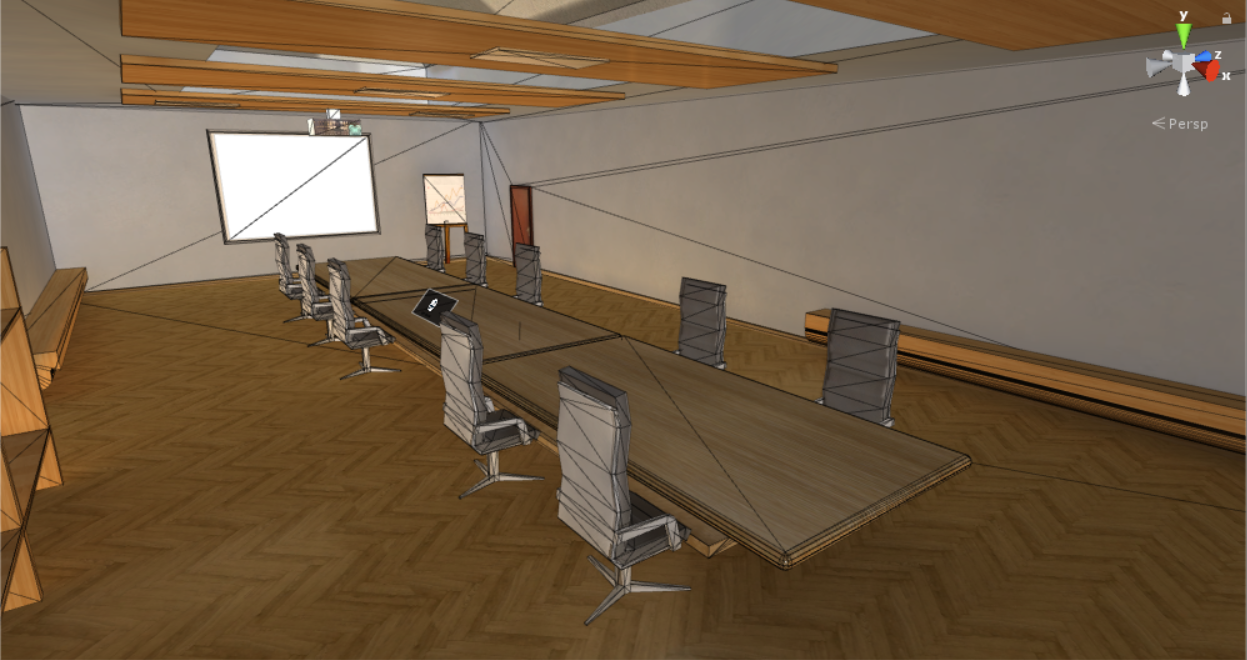
\includegraphics[width=0.65\textwidth]{figure/RoomWire}
	\centering
	\vspace{0.3cm}
	\caption{la visualizzazione della stanza non illuminata dall'editor con il \textit{wireframe} in evidenza (21k triangoli, 30k vertici) }
\end{figure}
Un'altro effetto che ho ottimizzato nella creazione della scena è l'\textit{overdraw}, ovvero quando oggetti sono renderizzati di fronte ad altri, sprecando le risorse della GPU. Per evitare che ciò accada tutte i modelli che non subiranno trasformazioni devono essere settati come \textit{static}, in particolare \textit{occluder static} e \textit{occludee static} in modo da poter generare dall'apposito pannello una mappa che contiene di dati relativi all'occlusione. Questi dati permettono anche di risparmiare non renderizzando gli oggetti fuori dal campo visivo (\textit{Occlusion Culling}).
\begin{figure}[H]
	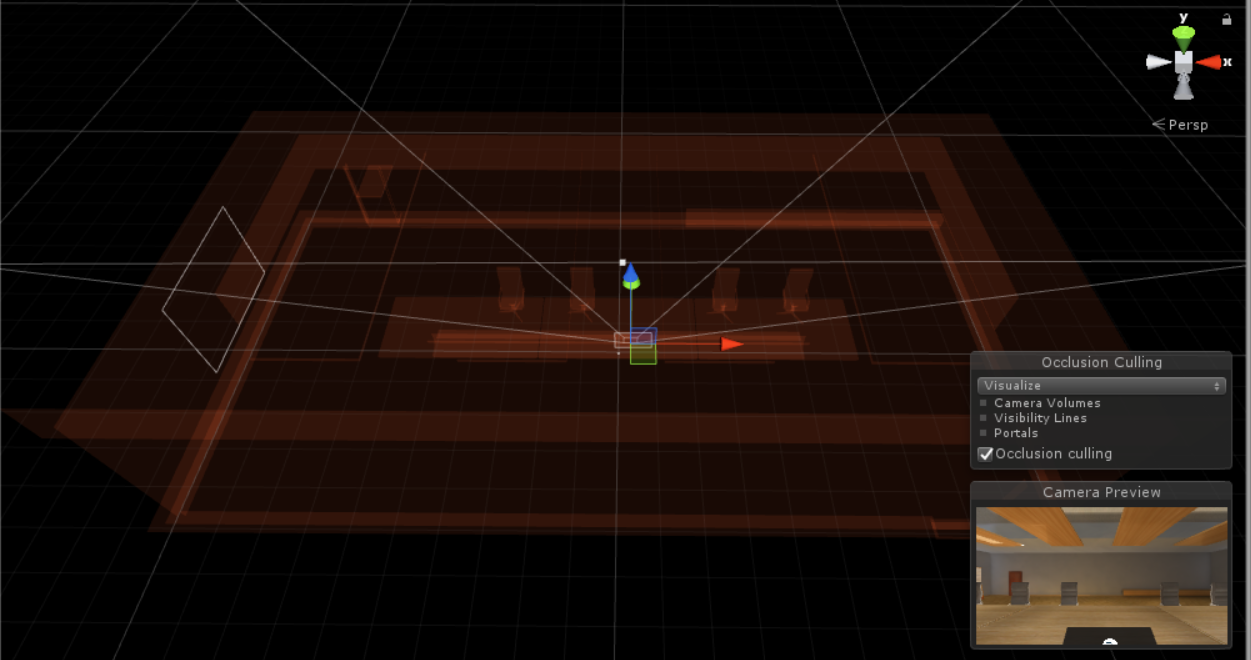
\includegraphics[width=0.65\textwidth]{figure/Overdraw}
	\centering
	\vspace{0.3cm}
	\caption{questa figura mostra la visualizzazione dell'\textit{overdraw}: nei punti in cui i modelli vengono sovrapposti, l'arancione si fa più intenso. Da notare l'assenza delle poltrone fuori dal capo visivo della telecamera (linee bianche).}
\end{figure}
Un'altro strumento che ho adoperato nel processo di ottimizzazione è il \textit{raggruppamento delle chiamate alle API grafiche (Draw Call Batching)}, spesso molto esigenti dal punto di vista delle risorse. Unity aiuta gli sviluppatori
offrendo due strumenti:
\begin{itemize}
	\item Raggruppamento dinamico (\textit{Dynamic Batching}): ottimale per piccole mesh, i cui vertici simili vengono raggruppati dalla CPU e renderizzati una volta sola. Se abusato può appesantire troppo la CPU.
	\item Raggruppamento statico (\textit{Static Batching}): combina GameObjects statici in uniche mesh più grandi, rendendo più veloce il processo di rendering. Può aumentare i costi di accesso memoria se usato troppo.
\end{itemize} 
Solamente oggetti che condividono gli stessi materiali possono essere raggruppati insieme, per questo ho cercato di utilizzarne pochi in tutta la scena creando delle \textit{texture atlases} in cui più texture sono unite formandone una più grande. Se i GameObject rispettano questo vincolo e non hanno \textit{mirroring}(un oggetto con scala +1 ed un altro con scala -1) nelle componenti \textit{transform} vengono raggruppati dinamicamente in automatico. Invece il vincolo affinché un oggetto venga raggruppato staticamente nella fase di rendering è che sia statico. \\

Probabilmente la parte che più grava sulle performance di un'applicazione è quella relativa all'illuminazione e questo è ancora più importante se si parla di realtà virtuale. L'illuminazione infatti deve essere calcolata precedentemente, poiché un approccio real time sarebbe troppo dispendioso per un dispositivo mobile. Quando questi atlanti dell'illuminazione (\textit{lightmaps}) sono calcolati a priori, gli effetti della luce sugli oggetti statici sono scritti sulle texture che verranno applicate alle geometrie, riproducendo l'illuminazione desiderata. Queste lightmaps possono includere sia la luce diretta che colpisce le superfici, sia quella indiretta che rimbalza tra le geometrie. L'unico limite è che le luci non possono cambiare a tempo di esecuzione. \\
Importanti ai fini di snellire il processo d'illuminazione della scena sono i \textit{light probes}. La loro unica differenza con le lightmaps è che invece di immagazzinare e usare le informazioni riguardanti la luce che colpisce delle superficie, gestisce la luce che passa per gli spazi vuoti nell'ambientazione, conferendo alla scena un'aspetto più naturale. \\
Infine per dare l'ultimo tocco di realismo alla scena ho utilizzato un \textit{reflection probe}, ovvero uno strumento che funge da camera che cattura un'immagine sferica di ciò che la circonda. Questa immagine è immagazzinata in una \textit{cubemap} la quale fornisce informazione ai materiali che riflettono o sono specchiati.\\

\begin{figure}[H]
	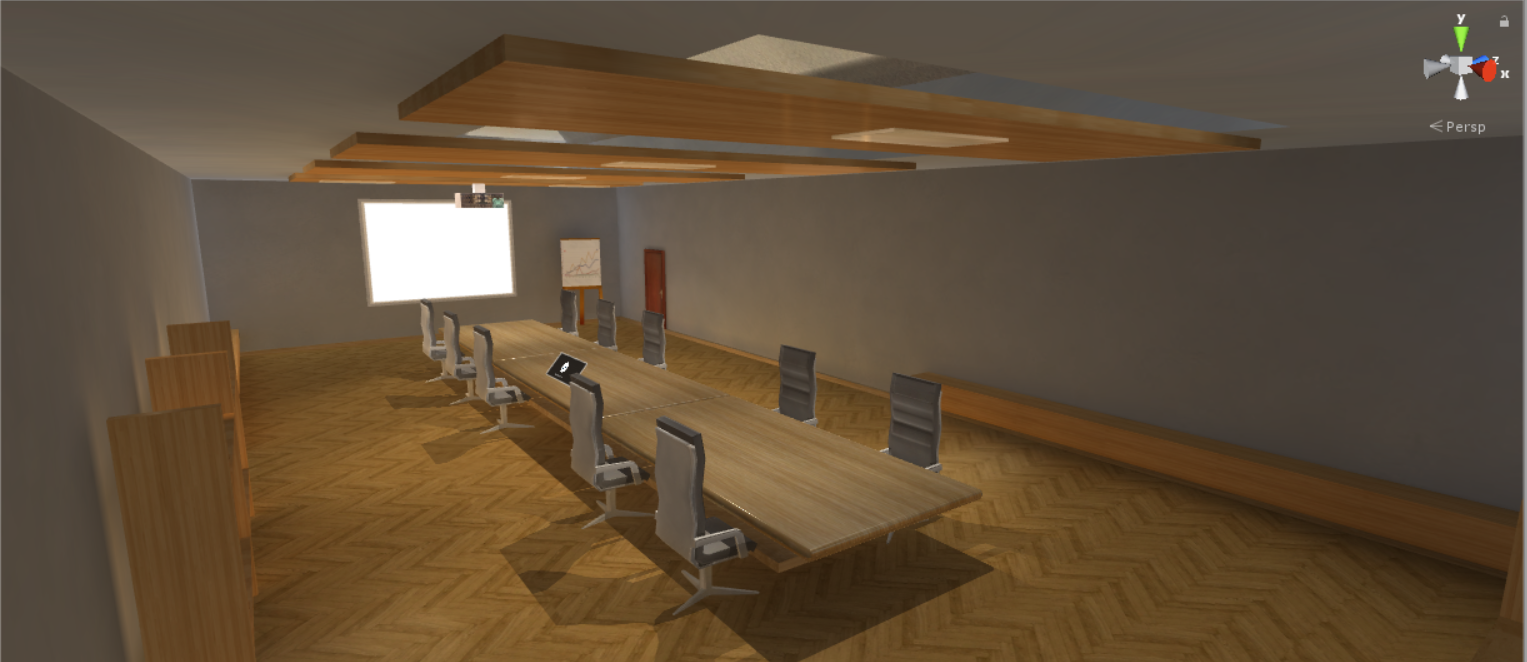
\includegraphics[width=0.85\textwidth]{figure/Lighted}
	\centering
	\vspace{0.3cm}
	\caption{L'ambientazione finale con la corretta illuminazione.}
\end{figure}
\begin{figure}[H]
	\centering
	\begin{minipage}[b]{0.49\textwidth}
		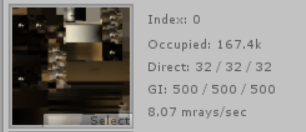
\includegraphics[width=\textwidth]{figure/Lightmap1}
		{\footnotesize \centerline{(a)} \par}
	\end{minipage}
	\hfill
	\begin{minipage}[b]{0.49\textwidth}
		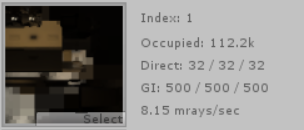
\includegraphics[width=\textwidth]{figure/Lightmap2}
		{\footnotesize \centerline{(b)} \par}
	\end{minipage}
	\begin{minipage}[b]{0.49\textwidth}
		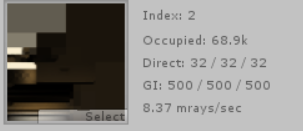
\includegraphics[width=\textwidth]{figure/Lightmap3}
		{\footnotesize \centerline{(b)} \par}
	\end{minipage}
	\caption{Le tre lightmaps computate da Unity contenenti le informazioni sulla luce salate in forma di texture atlases.}
\end{figure}
L'utilizzo di un filtro \textit{anti-aliasing} è altamente consigliato se si vogliono sviluppare applicazioni VR, poiché aiuta a "levigare" l'immagine evitando la presenza di bordi frastagliati. In particolare per le esperienze con i Gear VR è quasi obbligatorio l'adozione di un filtro MSAA, ai fini di ottenere una buona esperienza per l'utente. \\

Infine rendere efficiente la computazione della GPU si deve tenere in considerazione che tipo di \textit{shader} si utilizza. Essi sono piccoli script che contengono i calcoli matematici e gli algoritmi che computano il colore di ogni pixel renderizzato basandosi sulle informazioni della luce e dei materiali. Posso fungere da collo di bottiglia del processo di ottimizzazione. Nel caso di questo progetto mi sono servito degli \textit{shader} già presenti all'interno di Unity specializzati per operare su dispositivi mobili, in particolare il tipo \textit{unlit} che non gestisce la parte relativa alla luce, lasciando il compito alle lightmaps.

\newpage

\section{Interfaccia grafica}

Quando si progetta un'interfaccia grafica per un'esperienza VR ci sono diveri fattori da tenere in considerazione. La risoluzione dei Gear VR è di 2560 x 1440 (1280 x 1440 per occhio) può portare ad un effetto di pixelation, ovvero quando i singoli pixel diventano evidenti. Questo è particolarmente vero per elementi grafici di grandi dimensioni in cui è presente del testo.\\

Nelle applicazioni non immersive, la UI è spesso posizionata in cima e renderizzata per ultima davanti a tutti gli altri elementi, formando quello che si definisce un HUD (\textit{Heads Up Display}). Questo tipo di UI è riferita come un'interfaccia grafica \textit{non diegetica} , ovvero che non esiste nel mondo, ma ha senso per l'utente nel contesto dell'applicazione. Un'approccio simile si ha con la musica nelle opere cinematografiche. In Unity questo processo è applicabile scegliendo un \textit{canvas}  di tipo \textit{overlay} o \textit{camera} posizionata sullo spazio del display. In un'applicazione VR queste interfacce grafiche sono prive di senso, poiché seguirebbero il movimento della testa e le informazioni visualizzate sarebbero difficilmente messe a fuoco dai nostri occhi data la vicinanza degli schermi a quest'ultimi.\\

\begin{wrapfigure}{rH}{0.45\textwidth} %this figure will be at the right
	\centering
	\includegraphics[width=0.45\textwidth]{figure/diegetic}

\end{wrapfigure}


Dobbiamo puntare quindi ad un' UI \textit{spaziale}, ovvero posizionata nello spazio del mondo virtuale ed indipendente dai movimenti del visore. Questo permette una navigazione visiva tra gli elementi dei canvas semplice e naturale. L'interfaccia grafica quindi va considerata come parte integrante del mondo e deve essere coerente con esso. E' utile posizionare i canvas ad una distanza confortevole per la lettura, troppo vicino all'utente potrebbe ricreare i problemi descritti in precedenza. Un problema in ci si imbatti con questi tipi di UI è la perdita di controllo su cosa mostrare all'utente. Anche è possibile collegare i movimenti dell' UI a quelli della telecamera di modo da avere sempre davanti agli occhi le informazioni che dobbiamo visualizzare, questo metodo è consigliabile solo per elementi come puntatori o mirini che fanno concettualmente parte dell'utente e che gli permetto di interagire con il mondo, poichè potrebbe portare a una sensazione claustrofobica, per cui l'utente non può scrollarsi di dosso le informazioni e lo obblighiamo a guardarle. E' anche vero però che, avendo quest'ultimo una totale libertà di rotazione della testa, non possiamo costringerlo a guardare nella giusta direzione e potrebbe perdere informazioni o momenti importanti. Per risolvere questo inconveniente vanno progettati ambienti in cui fin dall'inizio è presa in considerazione la posizione dell'interfaccia grafica. Nel caso della sala riunione virtualizzata gestito il problema, più evidente nella fase iniziale in cui l'utente deve configurare il suo profilo, oscurando tutta la stanza ed illuminando con dei riflettori i due avatar e il canvas con il quale l'utente deve interagire. Portiamo così l'utilizzatore a trovare in modo naturale le informazioni cruciali ai fini dell'esperienza. 
\begin{figure}[H]
	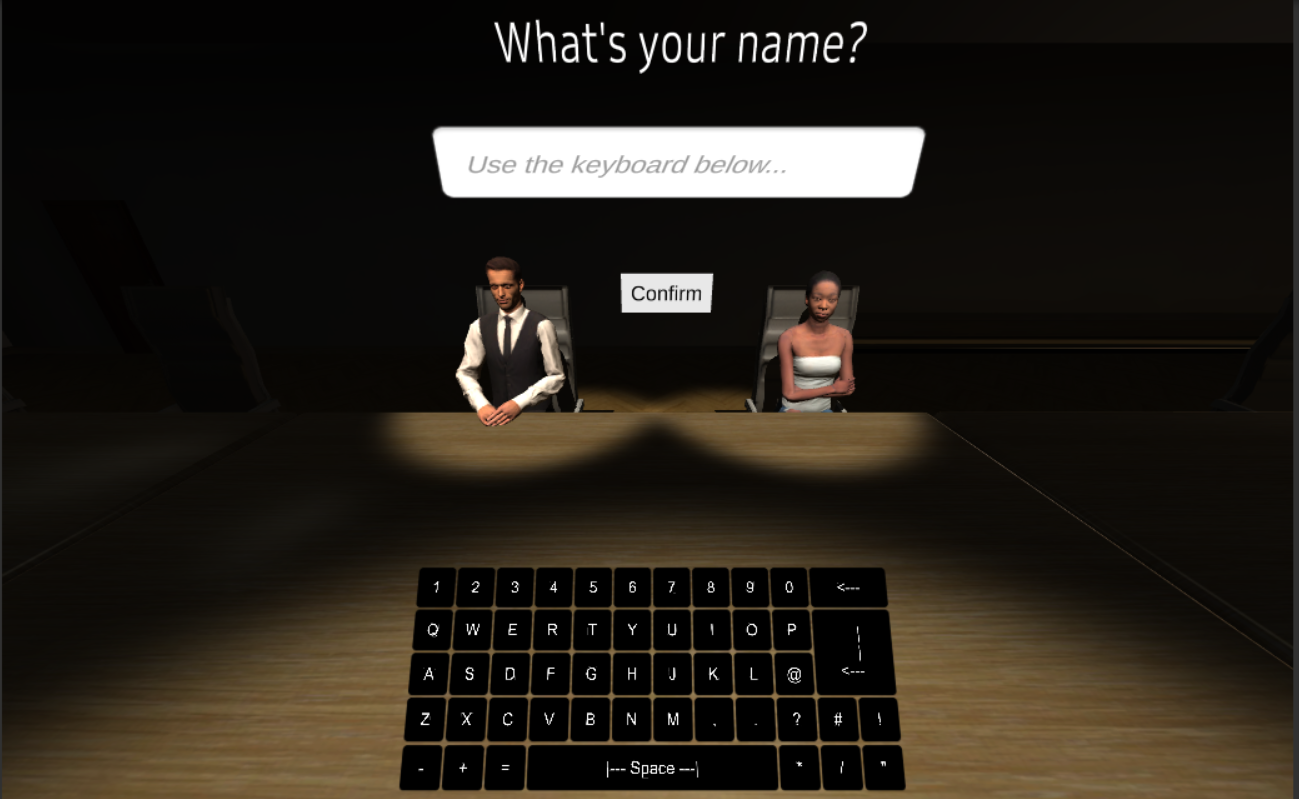
\includegraphics[width=0.85\textwidth]{figure/UIKeyboard}
	\centering
	\vspace{0.3cm}
	\caption{ Questa immagine ritrae il passo quattro del caso d'uso preso in considerazione. L'assenza di elementi distraenti porta a interagire con l'UI.}
\end{figure}

Per gestire l'inserimento dei dati e delle preferenze dell'utente ho utilizzato un'approccio diegetico, in cui i componenti grafici sono immersi nella scena. La tastiera ad esempio è composta da un'insieme di pannelli posizionati dinnanzi all'utente; la scelta degli avatar è gestita tramite l'inserimento di un canvas tra i modelli e il giocatore; I documenti nella sala riunioni sono condivisi su un proiettore rendendo più naturale l'utilizzo; il nome dell'utente è visualizzato sopra il suo avatar assieme ad altre icone che indicano se sta parlando o ha disattivato il microfono.     

\begin{wrapfigure}{rH}{0.35\textwidth} %this figure will be at the right
	\centering
	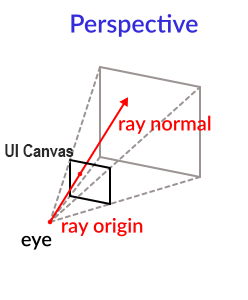
\includegraphics[width=0.25\textwidth]{figure/raycast}
	
\end{wrapfigure}

L'utente può interagire con questi menu in due modi: con l'utilizzo del controller ufficiale Gear VR (scelta consigliata); con l'utilizzo del touchpad presente sul visore e l'ausilio di un "mirino" che aiuta il puntamento; in entrambi i casi il processo di selezione è gestito attraverso dei \textit{collider}, componenti che gestiscono le interazioni fisiche, posizionati sui canvas che rilevano se il puntatore \textit{raycast} è posizionato su di esse. Se ciò avviene e si preme il pulsante di selezione (il grilletto del controller oppure un tocco sul touchpad) si chiamera il corrispettivo metodo che gestisce gli eventi associati al bottone. Ho generato una classe \textit{UIController} singleton, ovvero unica e che permane tra le varie scene, addetta alla gestione di tutte le interazioni con l'interfaccia grafica.



\section{Architettura Software}
Ora che l'applicazione ha un'ambientazione virtuale ottimizzata e delle interfacce grafiche configurate è necessario implementare le funzionalità.
\subsection{Librerie Esterne}
Per facilitarne lo sviluppo, il progetto implementa quattro librerie esterne principali. Due di queste gestiscono il visore e forniscono degli strumenti aggiuntivi per la creazione di applicazioni in realtà virtuale (\textit{Oculus SDK}, \textit{Virtual Reality Toolkit}); le altre due si occupano della connessione ad un server e della comunicazione realtime tra i due Gear VR (\textit{Photon Unity Networking}, \textit{Photon Unity Networking Voice}).\\

\begin{flushleft}
	\underline{\textit{Oculus SDK}:}
	Integrata già all'interno di Unity, questa libreria si interfaccia con le componenti hardware del visore fornendo delle API di base che gestiscono la renderizzazione in modalità stereo dei display, i bottoni fisici o gli eventuali controller e il tracciamento dei movimenti del visore. \cite{OculusDoc}
\end{flushleft}

\begin{flushleft}
	\underline{\textit{"VRTK"}:}
	E' una libreria estremamente utile poiché fornisce molteplici script e prefab che semplificano e arricchiscono gli strumenti di base forniti dalla SDK ufficiale di Oculus e funge da \textit{wrapper} di quest'ultimo.
	\cite{VRTK}
\end{flushleft}

\begin{flushleft}
	\underline{\textit{Photon Unity Networking}:}
	Gestisce la parte backend dell'applicazione. Offrono in un'opzione gratuita i loro server per la gestione real-time degli eventi, con un limiti imposti sul numero di utenti connessi contemporaneamente. Utile perchè fornisce una soluzione \textit{plug and play} adatta alle tempistiche del progetto dimostrativo. Per usufruirne bisogna registrare l'applicativo sul sito ufficiale.
	\cite{VRTK}
\end{flushleft}

\begin{flushleft}
	\underline{\textit{Photon Unity Networking Voice}:}
	Libreria gemella di quella appena descritta che offre un servizio di VOiP da utilizzare all'interno dell'applicazione.
	\cite{Photon}
\end{flushleft}
\subsection{Sviluppo}
\subsubsection{Configurazione della Realtà Virtuale}
Una volta importate le librerie descritte in precedenza e configurato il progetto per la realtà virtuale bisogna popolarlo con le componenti opportune. Come prima deve essere creato un oggetto vuoto a cui ho connesso lo script \textit{VRTK\_SDK Manager} che si occupa della configurazione delle SDK supportate. Questo oggetto è parent di un GameObject contenente lo script \textit{VRTK\_SDK Setup} nel quale va configurata la libreria da utilizzare, nel caso di questa applicazione quella relativa al Gear VR. A sua volta quest'ultimo GameObject, sarà parent del prefab fornitoci dalla SDK Oculus che gestisce il visore. \\
A questo punto è necessario connettere allo script \textit{VRTK\_SDK Manager} un'oggetto che fungerà da controller. Questo GameObject dovrà contenere la classe, fornita dalla libreria VRTK, \textit{"ControllerEvents"}, che gestisce gli eventi scaturiti dai diversi tipi di input. Oltre a questa ho implementato i seguenti script:
\begin{itemize}
	\item  \textit{Pointer}: permette la creazione e la renderizzazione del puntatore.
	\item  \textit{UI Pointer}: permette le interazioni con gli elementi dell'UI.

\end{itemize}
\begin{minipage}[h]{0.75\textwidth}
	\begin{itemize}
		\item \textit{Radial Menu}: permette di aumentare il numero di bottoni disponibili creandone alcuni virtuali e mostrandoli come un menu radiale renderizzato sopra il controller. Queste voci saranno rese visibili e accessibili scorrendo il dito sul touchpad del telecomando.
	\end{itemize}
\end{minipage}
\hfill
\begin{minipage}[h]{0.2\textwidth}
	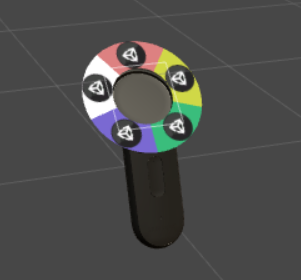
\includegraphics[width=\textwidth]{figure/radial}
	
\end{minipage}


\vspace{0.5cm}
Per poter visualizzare il controller dobbiamo inserire come figlio di questo GameObject una mesh.\\

Al termine di questi passaggi si ha un'applicazione in realtà virtuale funzionante all'interno dei visori Gear VR, in cui l'utente può guardarsi attorno e selezionare le voci dai menu.

\subsubsection{Gestione delle funzionalità in Rete}
Questa risulta essere la parte più delicata del progetto poiché lo scopo principale dell'applicazione è quello di permettere a più utenti di ritrovarsi nella sala riunioni attraverso la rete. \\

\begin{figure}[H]
	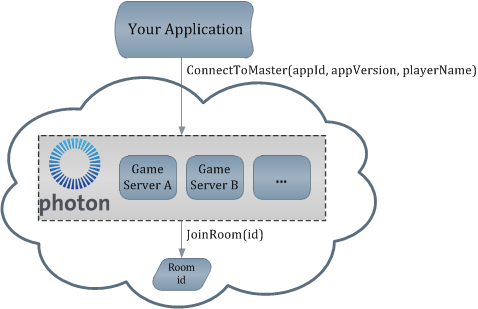
\includegraphics[width=0.50\textwidth]{figure/Photon}
	\centering
	\vspace{0.3cm}
	\caption{La gestione della connessione alla rete schematizzata.}
\end{figure}
\newpage
Per prima cosa bisogna stabilire una connessione con il server e creare una stanza utilizzato la libreria Photon Unity Networking. Per fare ciò è necessario creare una classe \textit{NetworkController} che gestisca questa parte. 
\begin{algorithm}
	\caption{Classe che gestisce la connessione con il server}
\begin{algorithmic}
	\STATE{\vspace{0.2cm}public class NetworkController : MonoBehaviour \{}\\
	\hspace{0.1cm}
	\bindent
		\STATE{private string m\_roomName = "VMR\_Test"}\\
			\STATE{\vspace{0.3cm} void Start() \{}
				\STATE{\vspace{0.1cm} \hspace{0.3cm} PhotonNetwork.ConnectUsingSettings("0.1"); }\\
			\hspace{0.1cm}
			\hspace{1.1cm}\}
			\STATE{\vspace{0.3cm}void OnJoinedLobby() \{}
				\STATE{\vspace{0.1cm} \hspace{0.3cm} RoomOptions roomOpt = new RoomOptions() \{maxPlayers = 4\};}
				\STATE{\hspace{0.3cm} PhotonNetwork.JoinOrCreateRoom(m\_roomName,roomOpt,TypedLobby.Default);}\\
				\hspace{0.1cm}
				\hspace{1.1cm}\}\\
				
			\STATE{\vspace{0.3cm} void OnJoinedRoom() \{}
				\STATE{ \vspace{0.1cm} \hspace{0.3cm} PhotonNetwork.Instantiate("NetworkedPlayer",Vector3.zero,Quaternion.identit,0);}\\
				\hspace{0.1cm}
				\hspace{1.1cm}\}
			\eindent
			\hspace{0.1cm}
\end{algorithmic}
\end{algorithm}


In questa classe definiamo una variabile di tipo stringa m\_roomName che sarà il nome della stanza che creeremo sul server. Questo parametro funge da "chiave" infatti con questo nome altri utenti potranno accedere alla stessa stanza. Essendo un'applicazione dimostrativa non ci preoccupiamo di generare un nome univoco e sicuro, vogliamo anzi che tutti gli utenti finiscano nella stessa stanza. \\
Il metodo ConnectUsingSettings() si connette ai server offerti da Photon e creando una lobby pubblica e prende come parametro la versione dell'applicazione. Appena ci si connette alla lobby viene chiamata la callback OnJoinedLobby(), la quale sovrascriviamo nella classe. Al suo interno infatti prima gestiamo le opzioni della stanza(numero di utenti massimi, visibilità, ecc.) poi la creiamo se non ne esiste un'altra con lo stesso nome, altrimenti proviamo ad unirci a quella esistente. Qualora riuscissimo ad entrare verrà attivata un'altra callback: OnJoinedRoom(). Nel nostro caso dobbiamo istanziare a lato server, un prefab dell'utente ("NetworkedPlayer") specificandone posizione e rotazione.\\

Dobbiamo ora scrivere lo script NetworkPlayer che collegheremo ad un avatar 3D. Questa classe estende Photon.MonoBehaviour che ci fornisce gli strumenti necessari per la sincronizzazione real time. Quando viene istanziata, disattiva localmente il modello 3D del suo avatar, il quale altrimenti ostruirebbe la vista all'utente. Procede poi  scegliendo il posto da occupare attorno al tavolo della sala riunioni a seconda del valore assunto dalla variabile countOfPlayersInRooms che indica quante persone sono già connesse. Se la connessione va a buon fine, attiva le due componenti relative alla chat vocale: \textit{Photon Voice Speaker} e \textit{Photon Voice Recorder}. Queste si collegano ad un server separato, e si occupano del funzionamento del servizio di VOiP, registrando la voce e inviandola a tutti i membri della stanza. In questo caso ho sovrascritto alcuni metodi della classe "Photon Voice Recorder" per inserire la funzionalità \textit{push-to-talk}, con la quale solo con la pressione di un specifico pulsante si può attivare la chat vocale, evitando fastidiosi rumori ambientali.\\
Un'altra componente fondamentale dell'oggetto è definita PhotonView. Grazie a questa infatti il server sa che deve aggiornare per tutti i client i movimenti e le rotazione compiuti dal GameObject, che nel nostro caso sono proprio i movimenti del capo dell'utente.

A questo punto due utenti possono entrare nella sala riunioni virtuale, vedere i rispettivi movimenti della testa e comunicare attraverso una chat vocale.

\
L'ultima parte che rimane da gestire è l'invio dei documenti ad altri dispositivi. Questa funzione non rientra totalmente nelle funzionalità di un motore grafico ed è stata la parte più complessa del progetto poiché Unity non fornisce nessuna libreria nè per navigare tra i dati del cellulare nè per l'invio di file sulla rete. Il mio approccio è stato quello di creare una classe "FileExplorer" che implementasse il codice nativo Android. Unity permette questo processo offrendo dei tipi di oggetto speciali denominati "\textit{AndroidJavaObject}", i quali fungono da wrapper per una classe nativa. Con l'aiuto della classe \textit{java.io.File} ho creato un semplice esplora risorse per navigare nelle cartelle del cellulare filtrando i file a seconda dell'estensione (pdf,doc,ecc.). \\ 

\begin{algorithm}
	\caption{L'algoritmo che gestisce la ricerca dei file PDF trovati nella cartella passata come parametro}
	\begin{algorithmic}
		\STATE{\vspace{0.2cm}AndroidJavaObject dir=GetExternalStoragePublicDirectory(DirectoryName);}\\
		
		\STATE{ \vspace{0.1cm} AndroidJavaObject[] files=directory.Call<AndroidJavaObject[]>("listFiles");}\\
		\STATE{\vspace{0.1cm} List<AndroidJavaObject> filteredFiles = new List<AndroidJavaObject>();}\\
		\FOR{AndroidJavaObject file in files}
		\IF{getFileExtension(file) == "pdf"}
		\STATE{filteredFiles.Add(file)}
		\ENDIF
		\ENDFOR
		\STATE{return filteredFiles;}
		
	\end{algorithmic}
\end{algorithm}



\newpage

Cliccando il documento che vogliamo trasferire si invia il percorso del file ad alla classe "FileConverter". Questa utilizza le classi \textit{nativeandroid.os.ParcelFileDescriptor}, \textit{java.io.FileOutputStream}, \textit{java.io.File}, \textit{android.graphics.pdf.PdfRenderer}, \\ \textit{android.content.Context}, \textit{android.graphics.Bitmap} per leggere il file, convertirlo nella rispettiva bitmap.

Quest'ultima si può finalmente inviare agli altri dispositivi all'interno di Unity utilizzando una \textit{RPC (Remote Procedure Calls)} ovvero degli eventi forniti da Photon che chiamano metodi su client remoti (ma nella stessa stanza). A questo punto ogni client riceve in forma parametrica la bitmap, la quale viene riscritta sotto forma di texture  dalle classi questa volta interne a Unity.\\
Qualora si volesse condividere sul proiettore un documento, premendo l'apposita voce nel menu spaziale, verrà attivata una RPC che mostrerà a tutti i presenti la stessa immagine sullo schermo. 
\begin{algorithm}
	\caption{L'algoritmo che gestisce l'invio dei dati con una chiamata RPC}
	\begin{algorithmic}
		\STATE{\vspace{0.2cm}[PunRPC] }\\
		
		\STATE{ \vspace{0.1cm} void ReciveByteArray(byte[] data) \{ }\\
		\STATE{\vspace{0.1cm} \hspace{0.1cm}Texture2D tex = new Texture2D(2000, 658,TextureFormat.PVRTC\_RGB4,false);}
		\STATE{\vspace{0.1cm} \hspace{0.1cm} tex.LoadRawTextureData(data);}	
		\STATE{\vspace{0.1cm} \hspace{0.1cm} Sprite sprite = Sprite.Create(tex,new Rect(0.0f,0.0f,tex.width,tex.height),new Vector2(0.5f, 0.5f),100.0f);}
		\STATE{\vspace{0.1cm} \hspace{0.1cm} return sprite}	
		\STATE{\vspace{0.1cm} \}}\\	
	\end{algorithmic}
\end{algorithm}
\begin{algorithm}
	\caption{L'algoritmo che gestisce la creazione di una Texture partendo dalla relativa Bitmap passata come parametro}
	\begin{algorithmic}
		\STATE{\vspace{0.2cm}MemoryStream msImage = new MemoryStream();}\\
		
		\STATE{ \vspace{0.1cm} \_bitmap.Save(msImage, \_bitmap.RawFormat);}\\
		\STATE{\vspace{0.1cm} newTexture.LoadImage(msImage.ToArray());}\\
		\STATE{\vspace{0.1cm} SpriteRenderer newSprite;}
		\STATE{\vspace{0.1cm} newSprite.material.maiTexture = newTexture;}
		\STATE{\vspace{0.1cm} return newSprite;}
		
	\end{algorithmic}
\end{algorithm}

A questo punto dello sviluppo l'applicazione implementa tutte le funzionalità descritte nel caso d'uso descritto in precedenza. L'utente, avviata l'applicazione e indossato il visore si ritrova immerso, in un ambiente virtuale, nel quale ha la possibilità di personalizzare le caratteristiche base del suo profilo. Può creare una sala riunione o connettersi ad una già esistente. In quest'ultima è rappresentato da un avatar che segue i suoi movimenti e può parlare o condividere documenti con altri utenti.









